\documentclass[11pt]{article}
\usepackage[utf8]{inputenc}
\usepackage[T1]{fontenc}
\usepackage{amsmath,amssymb,amsthm}
\usepackage{graphicx}
\usepackage{booktabs}
\usepackage{float}
\usepackage{hyperref}
\usepackage{xurl}
\usepackage[margin=1in]{geometry}
\usepackage{caption}

\hypersetup{colorlinks=true, linkcolor=blue, citecolor=blue, urlcolor=blue}

% Les figures sont dans paper/figures/, pas dans le dossier courant.
% Sans cette ligne, \includegraphics{fig1.pdf} ne trouve rien et LaTeX
% dessine un cadre vide avec le nom du fichier a la place du graphique.
% Dossier courant d'abord (donc aussi si les figures sont remplies a plat).
\graphicspath{{figures/}{}}

% ======================================================================
\newcommand{\AuthorNames}{BERRAMDANE Reddouane}
\newcommand{\AuthorAffiliations}{Independent Researcher}
\newcommand{\AuthorEmail}{reddoma@gmail.com}
\newcommand{\RepoURL}{https://github.com/reddoma742/prime-gaps-autocorrelation}
\newcommand{\ArxivID}{arXiv:XXXX.XXXXX}
% ======================================================================

\title{Persistent Negative Lag-One Dependence in Locally Detrended\\
Prime-Gap Windows up to $N = 10^9$, with Absence of Significant Positive
Autocorrelation up to $K = 1024$}

\author{\AuthorNames\\ \small \AuthorAffiliations\\ \small \texttt{\AuthorEmail}}
\date{September 2026}

\begin{document}
\maketitle

% ======================================================================
\begin{abstract}
We study the autocorrelation of consecutive prime gaps
$g_n = p_{n+1} - p_n$ using an exact segmented sieve up to $N = 10^9$,
yielding $50{,}847{,}532$ even gaps (excluding the initial odd gap
$g_1 = 3 - 2 = 1$). We show that the lag-one autocorrelation
$\rho_1$ of the locally detrended gap sequence is negative in every one
of ten logarithmic windows spanning $[10^4, 10^9)$, with moving-block
bootstrap 95\% confidence intervals excluding zero in every window. The
magnitude decays approximately monotonically from $\rho_1 \approx -0.095$
in the smallest window to $\rho_1 \approx -0.031$ in the largest,
consistent with a power law $|\rho_1| \sim (\log p)^{-c}$. A weighted
fit on the 8-window subset ($\log p \ge 12$) gives a point estimate
$c = 1.28 \pm 0.05$ (statistical) with bootstrap 95\% CI $[1.14, 1.57]$;
varying the window set produces estimates in $[1.26, 1.57]$, indicating
systematic sensitivity to the choice of subset. The quadratic decay ($c = 2$) is excluded in every
window-set choice tested, at $3.7\sigma$ to $14.4\sigma$, and at
$6.6\sigma$ on the bootstrap scale. The naive
logarithmic decay ($c = 1$) is excluded at $5.6\sigma$ using the
weighted-fit standard error, but only at $\approx 2.5\sigma$ on the
bootstrap scale of that same fit ($\mathrm{SE}_{\text{boot}} \approx
0.11$), at $2.6\sigma$ under the unweighted 8-window fit,
$4.1$--$4.3\sigma$ under the two 6-window fits, and $4.9\sigma$ under
the all-10-window fit: the exclusion holds for
every window set we tested, but with a margin ranging from marginal
($\approx 2.5\sigma$) to clear ($5.6\sigma$), and should be read as
suggestive rather than decisive.
Extending the analysis to $K = 1024$ lags on the globally detrended
sequence $\delta_n = g_n - \log p_n$, we find \textbf{no significant
positive autocorrelation at any individual lag}: only 255 of 1024 lags
are positive (24.9\%), the largest positive value is
$+3.86 \times 10^{-4}$, below the Bonferroni threshold of
$5.70 \times 10^{-4}$ by a factor of 0.68. A companion analysis of the
raw (non-detrended) global autocorrelation reveals a non-stationarity
artifact that produces 1016 of 1024 positive lags, with maximum value
$+4.24 \times 10^{-3}$ exceeding the threshold by a factor of 7.45;
this artifact disappears entirely upon detrending.

We also report a direct test of the Lemke Oliver--Soundararajan (LO-S)
conjecture mod 3: the ``stay'' probability
$P(p_{n+1} \equiv a \mid p_n \equiv a)$ for $a \in \{1, 2\}$ is
$0.44509$ and $0.44514$ respectively, deviating from $1/2$ by
approximately $-0.055$ at a $z$-score of approximately $-553\sigma$.
The
suppression is the same in both residue classes (the difference
corresponds to $z = 0.33$), but the corresponding conditional
autocorrelations differ between $a = 1$ and $a = 2$ by $3.6$--$4.5$
standard errors at $k = 1, 2, 3$; the symmetry is therefore
approximate. This is
the strongest signal in the paper, and it confirms the LO-S bias for
mod~3; a
quantitative test of the conjectured per-class constants is left
open. Within the largest window, the lag-$k$ autocorrelations satisfy
$\rho_k \approx \rho_1/k$ for $k \le 5$ to within $8\%$; the ratio
remains approximately monotone at higher lags but with increasing
deviation.

An inclusion--exclusion extension of the naive Hardy--Littlewood
pair-density heuristic reproduces the observed pair ratios to within
0.37\% mean absolute error --- a nearly tenfold ($9.6\times$)
improvement --- without any
fitted constants. As a byproduct of the analysis, the telescoping
identity for $\delta_n$ yields $\psi(10^9) - 10^9 = +1{,}595.99$,
consistent with the explicit bounds of B\"uthe.\footnote{Computed by
direct enumeration of the primes below $10^9$ rather than inferred from
the gap sequence, and quoted conservatively; the computed value is
$+1{,}595.9904$ and its precision is stated once, in Appendix~A.}
\end{abstract}

\noindent\textbf{Keywords}: prime gaps, autocorrelation,
Hardy--Littlewood, Lemke Oliver--Soundararajan, non-stationarity, block
bootstrap, Chebyshev function.

% ======================================================================
\section{Introduction}

\subsection{Motivation}
The prime numbers, though defined deterministically, exhibit
statistical regularities that have been studied for more than a
century. A central object in this study is the sequence of consecutive
gaps
\begin{equation}
g_n = p_{n+1} - p_n, \qquad n \ge 1,
\end{equation}
where $p_n$ denotes the $n$-th prime. The average size of $g_n$ grows
logarithmically: $\mathbb{E}[g_n] \sim \log p_n$, a fact already
implicit in the prime number theorem and made quantitative by the
classical heuristic of Cram\'er \cite{Cramer1936}, and refined in the
study of primes in short intervals \cite{Gallagher1976,Maier1985}
and in the asymptotic distribution of primes
\cite{Granville1995}. Whether consecutive
gaps behave as independent random variables, however, has been a
subject of long-standing interest.

The classical Hardy--Littlewood heuristic \cite{HL1923} predicts, for
any admissible pair of shifts $(a, b)$, a pair-correlation function of
the form
\begin{equation}
R_{\mathrm{HL}}(a,b) =
\frac{\mathfrak S(\{0,a,a+b\})}
     {\mathfrak S(\{0,a\})\,\mathfrak S(\{0,b\})},
\end{equation}
where $\mathfrak S(D) = \prod_p (1 - \nu_D(p)/p)(1-1/p)^{-k}$ is the
singular series associated with the pattern $D = \{d_1, \dots, d_k\}$,
and $\nu_D(p)$ is the number of distinct residues modulo $p$ occupied
by $D$.

\subsection{Recent developments}
The picture changed substantially with the work of Lemke Oliver and
Soundararajan \cite{LOS2016}, who discovered an unexpected bias in the
distribution of consecutive primes modulo a fixed modulus $q$: patterns
in which the two primes are congruent modulo $q$ are suppressed relative
to non-congruent patterns, with a bias of order $\log\log x / \log x$.
Such effects belong to the broader family of systematic biases among
the primes, alongside prime number races \cite{GranvilleMartin2006} and
Chebyshev's bias \cite{RubinsteinSarnak1994}.

The LO-S discovery raises a natural question for the gap sequence
itself: is $g_n$ correlated with $g_{n+1}$? The expected correlation,
if any, should be negative. Yet measuring it reliably at large $N$ is
complicated by (1) non-stationarity of the mean, and (2) the choice of
window and detrending.

\subsection{Our contribution}
In this paper we report a systematic, windowed analysis of the
autocorrelation of consecutive prime gaps up to $N = 10^9$. Main
contributions:
\begin{enumerate}
\item A cleanly measured approximately monotone decay of $\rho_1$ over
      ten windows, with weighted point estimate $c = 1.28 \pm 0.05$.
\item Absence of significant positive autocorrelation at any individual
      lag up to $K = 1024$ in the detrended sequence.
\item Identification and correction of a non-stationarity artifact.
\item Direct confirmation of the LO-S bias mod 3 at $|z| > 550\sigma$.
\item Ratio structure $\rho_k \approx \rho_1/k$ in the largest window.
\item Inclusion--exclusion pair-ratio model with 0.37\% mean absolute
      error.
\item A byproduct of the telescoping identity: the pipeline yields
      $\psi(10^9) - 10^9 = +1{,}595.99$, confirmed by direct
      enumeration of the primes below $10^9$, and consistent with the
      published explicit bounds for $\psi(x)$.
\item Reproducibility and AI disclosure (Section~\ref{sec:ack}).
\end{enumerate}

\subsection{Relation to prior work}
Negative correlations between consecutive prime gaps have been noted
empirically before (see \cite{Brent1974} and references therein), as
have exceptionally long gaps \cite{Ford2018} and, by a different
method, multiscale order in the primes \cite{Torquato2018}. Our
work extends those observations: (i) to a substantially larger range;
(ii) with a windowed, detrended methodology; (iii) with explicit
quantification of $c$; and (iv) with a direct, high-precision
confirmation of the LO-S bias mod 3.

\subsection{Structure}
Section~\ref{sec:data} defines the gap sequence, windows, and
estimator. Section~\ref{sec:protocol} describes the statistical
protocol. Section~\ref{sec:global} contrasts global and windowed
analyses, and reports the $K = 1024$ correlogram. Section~\ref{sec:main}
presents the main result. Section~\ref{sec:mod3} reports the mod-3
conditional autocorrelations and the direct LO-S test.
Section~\ref{sec:scaling} estimates $c$. Section~\ref{sec:pair}
discusses pair ratios. Section~\ref{sec:limits} lists limitations and
reproducibility details. Section~\ref{sec:ack} acknowledges
contributions and provides the AI disclosure. Appendix~A derives the
telescoping identity. Appendix~B provides a synthetic demonstration of
the non-stationarity artifact. Appendix~C reports a synthetic-null
control for the detrending.

% ======================================================================
\section{Data and Definitions}\label{sec:data}

\subsection{Prime gap sequence}
Let $p_n$ denote the $n$-th prime, with $p_1 = 2$. For $N = 10^9$:
\begin{equation}
\pi(10^9) = 50{,}847{,}534, \qquad n_{\text{gaps}} = 50{,}847{,}532,
\label{eq:ngaps}
\end{equation}
with mean gap $\bar g = 19.6666\ldots$. The value of $n_{\text{gaps}}$
equals $\pi(10^9) - 2$ because the analysis excludes the initial odd
gap $g_1 = 3 - 2 = 1$; the remaining gaps are all even.

\subsection{Sieve}
All primes up to $N$ were generated using an exact segmented sieve of
Eratosthenes in C++17. The sieve was validated against the known count
$\pi(10^9) = 50{,}847{,}534$ \cite{OEIS_A006880}. The reference
values are those tabulated in the On-Line Encyclopedia of Integer
Sequences \cite{OEIS} and, independently, in the published tables of
$\pi(x)$ of Oliveira e Silva \cite{OliveiraSilva2007}. The full pipeline
required approximately 22 hours on a 4-thread workstation.

\subsection{Logarithmic windows}
We partition the range into logarithmic windows
$W_i = [L_i, U_i)$ with $L_i, U_i \in \{10^k, 3\cdot 10^k\}$.

\begin{table}[H]\centering
\caption{Logarithmic windows and gap counts ($N = 10^9$).}
\label{tab:windows}
\begin{tabular}{lccl}
\toprule
Window $W_i$ & $m_i$ (gaps) & $\bar g_i$ & $\log p_i$ \\
\midrule
$[10^4, 3\times10^4)$         & 2,016     & 9.92  & 9.76  \\
$[3\times10^4, 10^5)$         & 6,347     & 11.03 & 10.91 \\
$[10^5, 3\times10^5)$         & 16,405    & 12.19 & 12.06 \\
$[3\times10^5, 10^6)$         & 52,501    & 13.33 & 13.21 \\
$[10^6, 3\times10^6)$         & 138,318   & 14.46 & 14.36 \\
$[3\times10^6, 10^7)$         & 447,763   & 15.63 & 15.52 \\
$[10^7, 3\times10^7)$         & 1,193,280 & 16.76 & 16.67 \\
$[3\times10^7, 10^8)$         & 3,903,596 & 17.93 & 17.82 \\
$[10^8, 3\times10^8)$         & 10,490,870 & 19.06 & 18.97 \\
$[3\times10^8, 10^9)$         & 34,595,208 & 20.23 & 20.12 \\
\bottomrule
\end{tabular}
\end{table}

\subsection{Autocorrelation estimator}
For a sequence $x_1, \ldots, x_m$, we define the lag-$k$ sample
autocorrelation as
\begin{equation}
\hat\rho_k =
\frac{\frac{1}{m-k}\sum_{i=1}^{m-k}(x_i - \bar x)(x_{i+k} - \bar x)}
     {\frac{1}{m}\sum_{i=1}^{m}(x_i - \bar x)^2},
\end{equation}
with $\bar x = \frac{1}{m}\sum_{i=1}^{m}x_i$.

\subsection{Detrending}
Within each window $W_i$, we fit
\begin{equation}
g_n = \alpha_i + \beta_i \log p_n + \varepsilon_n, \qquad p_n \in W_i,
\end{equation}
and define $\tilde g_n = g_n - (\hat\alpha_i + \hat\beta_i \log p_n)$.
For the global analysis, $\delta_n = g_n - \log p_n$.

\subsection{Conditional sequences}
For the mod-3 analysis:
\begin{equation}
g^{(1)}_n = \{g_n : p_{n+1} \equiv 1 \bmod 3\}, \quad
g^{(2)}_n = \{g_n : p_{n+1} \equiv 2 \bmod 3\}.
\end{equation}
The partition is on the closing prime $p_{n+1}$, and the two classes
together contain $|g^{(1)}| + |g^{(2)}| = \pi(10^9) - 2 = 50{,}847{,}532$
gaps, which is $n_{\text{gaps}}$ of
Eq.~\eqref{eq:ngaps}. It does not equal $\sum_i m_i =
50{,}846{,}304$, the total of Table~\ref{tab:windows}, because the ten
windows cover $p \geq 10^4$ only: the $1{,}228$ gaps opened at the
$1{,}229$ primes below $10^4$ lie outside every window. The
corresponding LO-S
contingency table (Section~\ref{sec:mod3}) conditions on the opening
prime and excludes the initial pairs involving $2$ and $3$, giving
$n_{\text{pairs}}(1) + n_{\text{pairs}}(2) = \pi(10^9) - 3 =
50{,}847{,}531$, consistent with Table~\ref{tab:los}.

\subsection{Notation summary}
\begin{table}[H]\centering
\begin{tabular}{ll}
\toprule
Symbol & Meaning \\
\midrule
$p_n$ & $n$-th prime \\
$g_n = p_{n+1} - p_n$ & $n$-th prime gap \\
$\delta_n = g_n - \log p_n$ & globally detrended gap \\
$\tilde g_n$ & locally detrended gap \\
$N$ & sieve limit ($N = 10^9$) \\
$\rho_k$ & lag-$k$ autocorrelation \\
$W_i$ & $i$-th logarithmic window \\
$m_i$ & number of gaps in $W_i$ \\
$c$ & descriptive exponent \\
\bottomrule
\end{tabular}
\end{table}

\subsection{Software and data}
C++ pipelines: \texttt{wheel\_\allowbreak analysis\_\allowbreak
v9\_\allowbreak 1\_\allowbreak complete.cpp},\\
\texttt{wheel\_\allowbreak analysis\_\allowbreak v10\_\allowbreak
supplement\_\allowbreak v2.cpp}, and
\texttt{theta\_\allowbreak powers.cpp}.
Python: \texttt{fit\_c.py}, \texttt{make\_\allowbreak figures.py},
\texttt{make\_\allowbreak appendix\_\allowbreak b.py},
\texttt{delta\_\allowbreak mean\_\allowbreak verify.py},
\texttt{compute\_\allowbreak psi.py}.
All code, CSV outputs, and a \texttt{README} are available at
\url{\RepoURL}.

% ======================================================================
\section{Statistical Protocol}\label{sec:protocol}

\subsection{Moving-block bootstrap}
Following K\"unsch \cite{Kunsch1989}, Hall--Horowitz--Jing
\cite{HHJ1995}, and the standard treatment of resampling for
dependent data \cite{Lahiri2003}, we fix block length
$\ell = \lceil n^{1/3}\rceil$, draw
$B = 5{,}000$ bootstrap samples, and form percentile confidence
intervals.

\subsection{Permutation test}
We perform a permutation test on the first $K = 10$ lags of the global
gap sequence with $P = 2{,}000$ random permutations. Minimum attainable
two-sided $p$-value: $p_{\min} = 1/2001 \approx 4.998 \times 10^{-4}$.

\noindent\textbf{Results.} The released file
\texttt{permutation\_v9\_1.csv} reports two-sided $p$-values equal to
the floor $p_{\min}$ for $k = 1, \ldots, 8$ and for $k = 10$, so eight
of the ten lags are significantly \emph{negative} and one, $k = 10$, is
significantly positive. The remaining lag, $k = 9$, gives
$p = 0.02849$: not significant at the Bonferroni-corrected level, but
significant under false-discovery-rate control. The observed values run
$\hat\rho_1 = -0.027532$, decaying in magnitude to
$\hat\rho_8 = -0.000588$, and then change sign,
$\hat\rho_9 = +0.000303$ and $\hat\rho_{10} = +0.000755$. The
permutation null has mean $\approx 0$ and standard deviation
$\approx 1.40 \times 10^{-4}$ at every lag, agreeing with the global
white-noise value $1/\sqrt{n_{\text{gaps}}} = 1.4024 \times 10^{-4}$
used in the next subsection. One point of interpretation must be
stated, since a naive comparison would be misleading. The positively
significant value at $k = 10$, $+7.55 \times 10^{-4}$, does exceed the
$K = 1024$ Bonferroni threshold of the next subsection (by a factor
$1.32$). This is not a contradiction of the $K = 1024$ analysis of
Section~\ref{sec:global}, for two reasons. First, that threshold is
derived for the detrended sequence $\delta_n$, whereas the permutation
test is run on the raw gaps $g_n$; on the raw sequence the threshold is
exceeded systematically at high lags, which is the non-stationarity
artifact of Section~\ref{sec:global} and Table~\ref{tab:k1024raw},
where $1016$ of $1024$ lags are positive. Second, $k = 10$ is a
single lag out of $1024$, and the artifact does not survive
detrending. Finally, the test covers $k \leq 10$ only and is silent on
the remaining $1014$ lags.

\subsection{Bonferroni correction}
At $\alpha = 0.05$: $\alpha/(2K)$ per tail, $\alpha/K$ per test.
For $K = 1024$: $z_{1-\alpha/(2K)} \cdot \mathrm{SE} \approx 4.061 \cdot
\mathrm{SE}$, with $\mathrm{SE} = 1/\sqrt{n_{\text{gaps}}} = 1.4024
\times 10^{-4}$, giving threshold $\approx 5.695 \times 10^{-4}$.
This white-noise standard error $\mathrm{SE} = 1/\sqrt{n_{\text{gaps}}}$
is used as a reference diagnostic. The exact finite-sample correction
for serial dependence is the Bartlett factor
$1 + 2\sum_{j \geq 1}\rho_j^2$ \cite{Bartlett1946}, which is
$\geq 1$ regardless of the sign of the autocorrelations. Using the
released $\delta_n$ correlogram up to $K = 1024$, this factor is
$\approx 1.0034$, so the
effective standard error is larger than the white-noise value by only
$\approx 0.17\%$; the Bonferroni threshold is correspondingly raised
from $5.695 \times 10^{-4}$ to approximately $5.705 \times 10^{-4}$.
The conclusions below are unaffected, since the largest positive value
of the $\delta_n$ correlogram is $3.86 \times 10^{-4}$.
The Bonferroni correction applies to significance thresholds across lags,
not to the construction of the bootstrap confidence intervals.
We do not report a Bartlett confidence interval: the sequence is
non-stationary, and the variance factor above already quantifies what
the Bartlett correction would do to the thresholds.

\subsection{Random seeds}
Permutation: 42. Bootstrap: 7919. Window bootstrap: 1234. Bootstrap
for $c$: seed 42, $B = 2{,}000$.

% ======================================================================
\section{Global versus Windowed Correlations}\label{sec:global}

\subsection{The global analysis (raw gaps)}
Applying the estimator to the raw gap sequence over $[2, 10^9]$:
\begin{enumerate}
\item Negative values for $k = 1, \ldots, 8$, ranging from
      $\hat\rho_1 = -0.0275$ to $\hat\rho_8 = -0.0006$.
\item First positive at $k = 9$: $\hat\rho_9 = +3.03 \times 10^{-4}$.
\item First positive lag whose interval excludes zero: $k = 10$,
      $\hat\rho_{10} = +7.55 \times 10^{-4}$.
\item Broad positive plateau for $k \in [10, 64]$.
\end{enumerate}

\subsection{The non-stationarity artifact}
The positive plateau at $k \ge 10$ is an artifact of the deterministic
growth of the mean gap. See Appendix~B for a synthetic demonstration.

\subsection{Absence of significant positive autocorrelation at all lags up to $K = 1024$}

\begin{table}[H]\centering
\caption{Global correlogram of $\delta_n = g_n - \log p_n$ up to
$K = 1024$.}
\label{tab:k1024delta}
\begin{tabular}{lr}
\toprule
Quantity & Value \\
\midrule
Total lags           & 1024 \\
Positive lags        & \textbf{255} (24.9\%) \\
First positive lag   & $k = 160$ \\
Maximum positive     & $+3.86 \times 10^{-4}$ at $k = 688$ \\
Bonferroni threshold ($z = 4.0612$) & $5.70 \times 10^{-4}$ \\
Max / threshold      & \textbf{0.677} \\
Tail mean, $k \in [160, 1024]$ & $-7.03 \times 10^{-5}$ \\
\bottomrule
\end{tabular}
\end{table}

\begin{table}[H]\centering
\caption{Global correlogram of raw gaps $g_n$ up to $K = 1024$.}
\label{tab:k1024raw}
\begin{tabular}{lr}
\toprule
Quantity & Value \\
\midrule
Total lags           & 1024 \\
Positive lags        & \textbf{1016} (99.2\%) \\
First positive lag   & $k = 9$ \\
Maximum positive     & $+4.24 \times 10^{-3}$ at $k = 688$ \\
Max / threshold      & \textbf{7.45} \\
Tail mean, $k \in [160, 1024]$ & $+3.79 \times 10^{-3}$ \\
\bottomrule
\end{tabular}
\end{table}

% --- Correspondance figures/ <-> legendes (verifiee sur le titre interne de
% --- chaque PDF, 1 octobre 2026). Les noms de fichiers restent ceux
% --- produits par make_figures.py ; c'est l'ordre d'inclusion qui a ete
% --- corrige, pas les noms.
%     fig1.pdf = rho_1 vs log p ................ Figure~\ref{fig:rho1}
%     fig2.pdf = correlogram fenetre k <= 64 .... Figure~\ref{fig:corr64}
%     fig3.pdf = correlogram detrende K = 1024 . Figure~\ref{fig:delta1024}
%     fig4.pdf = correlogram brut K = 1024 ..... Figure~\ref{fig:raw1024}
%     fig5.pdf = pair ratios .................... Figure~\ref{fig:pairs}
\begin{figure}[H]\centering
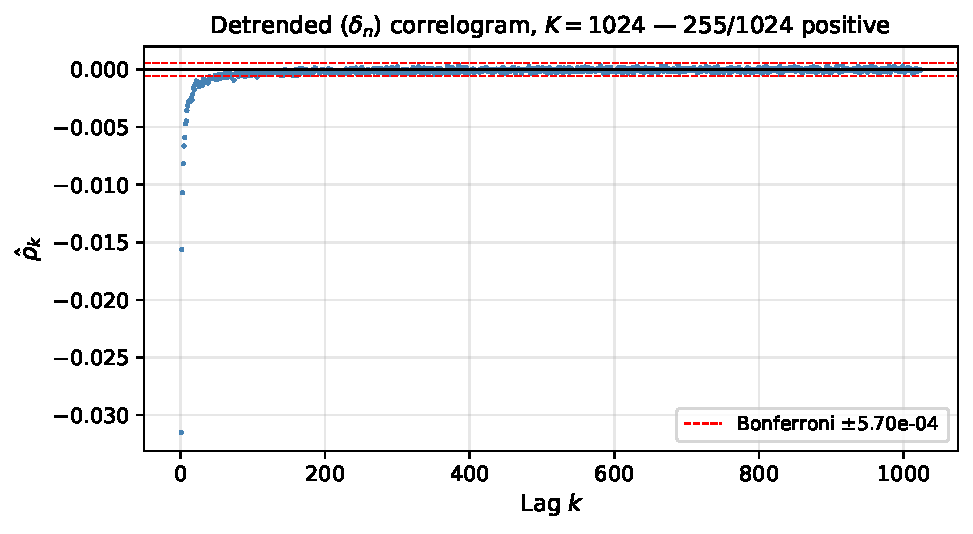
\includegraphics[width=0.85\textwidth]{fig3.pdf}
\caption{Detrended ($\delta_n$) correlogram up to $K = 1024$. Only
255/1024 lags are positive; all values fall below the Bonferroni
threshold (red dashed lines).}
\label{fig:delta1024}
\end{figure}

\begin{figure}[H]\centering
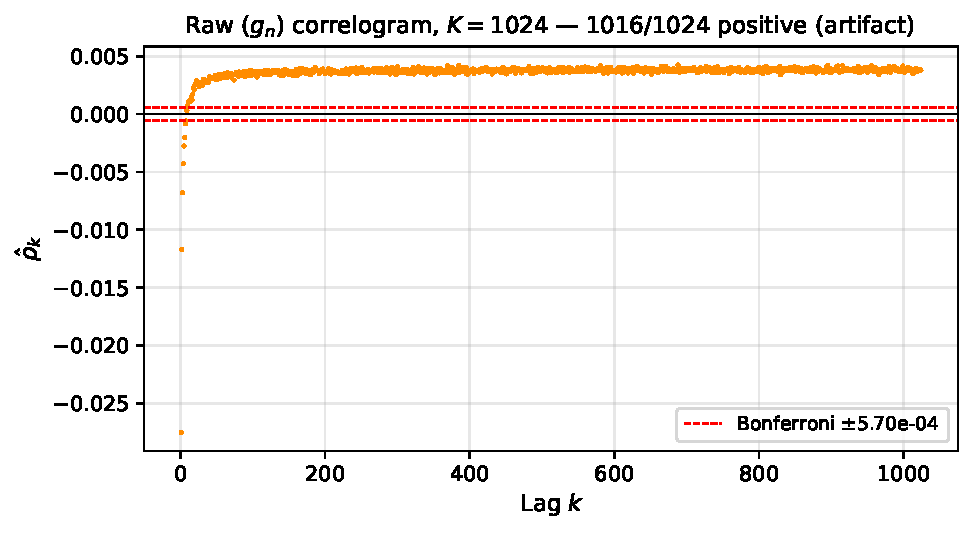
\includegraphics[width=0.85\textwidth]{fig4.pdf}
\caption{Raw correlogram, same range. 1016/1024 lags are positive, with
maximum exceeding the threshold by a factor 7.45 --- a non-stationarity
artifact that disappears upon detrending.}
\label{fig:raw1024}
\end{figure}

\noindent\textbf{Sign statistic.} The fraction of positive lags
(255/1024 = 24.9\%) deviates from the 50\% expected under a white-noise
null. Under a naive independent-lag model the deviation would
correspond to $z \approx 16\sigma$; however, the values of the
correlogram are serially dependent, and any small systematic offset in
the mean subtraction could also bias this fraction. A rigorous
estimate of significance would require an estimate of the effective
sample size of the correlogram, which we do not attempt here. We
therefore treat the sign statistic only as \emph{suggestive} of a weak
persistent negative bias, consistent with the windowed $\rho_1 < 0$
result of Section~\ref{sec:main}, and not as an independent
significance claim.

\subsection{Fourier constraint}
For any stationary sequence, non-negativity of the spectral density at
zero requires $1 + 2\sum_{k \ge 1}\rho_k \ge 0$. The partial sum using
the released $\delta_n$ correlogram over $k \in [1, 1024]$ is
$\sum_{k=1}^{1024}\rho_k = -0.247$, giving
$1 + 2 \cdot (-0.247) \approx 0.506 > 0$. The spectral constraint is
therefore satisfied with a wide margin across the observed range. We
note that the constraint in its strict form applies to a stationary
sequence; the globally detrended sequence $\delta_n$ is not strictly
stationary, so this check should be read as a diagnostic rather than a
formal verification.

% ======================================================================
\section{Main Windowed Result}\label{sec:main}

\subsection{Statement}
Across all ten logarithmic windows spanning $[10^4, 10^9)$, the
locally detrended lag-one autocorrelation is negative, with
moving-block bootstrap intervals excluding zero.

\begin{table}[H]\centering
\caption{Windowed lag-one autocorrelation. The 95\% intervals are
moving-block bootstrap percentile intervals; the Bonferroni correction
applies to significance thresholds, not to the intervals themselves.}
\label{tab:rho1}
\begin{tabular}{lrrrr}
\toprule
Window & $m_i$ & $\log p_i$ & $\hat\rho_1$ & Moving-block bootstrap 95\% CI \\
\midrule
$[10^4, 3\times10^4)$  & 2,016     & 9.76  & $-0.09490$ & $[-0.13299, -0.03794]$ \\
$[3\times10^4, 10^5)$  & 6,347     & 10.91 & $-0.08688$ & $[-0.10591, -0.06455]$ \\
$[10^5, 3\times10^5)$  & 16,405    & 12.06 & $-0.05579$ & $[-0.06895, -0.03987]$ \\
$[3\times10^5, 10^6)$  & 52,501    & 13.21 & $-0.05156$ & $[-0.05934, -0.04330]$ \\
$[10^6, 3\times10^6)$  & 138,318   & 14.36 & $-0.05188$ & $[-0.05650, -0.04658]$ \\
$[3\times10^6, 10^7)$  & 447,763   & 15.52 & $-0.04333$ & $[-0.04570, -0.04016]$ \\
$[10^7, 3\times10^7)$  & 1,193,280 & 16.67 & $-0.03793$ & $[-0.03938, -0.03593]$ \\
$[3\times10^7, 10^8)$  & 3,903,596 & 17.82 & $-0.03578$ & $[-0.03653, -0.03464]$ \\
$[10^8, 3\times10^8)$  & 10,490,870 & 18.97 & $-0.03277$ & $[-0.03311, -0.03199]$ \\
$[3\times10^8, 10^9)$  & 34,595,208 & 20.12 & $-0.03054$ & $[-0.03067, -0.03004]$ \\
\bottomrule
\end{tabular}
\end{table}

\begin{figure}[H]\centering
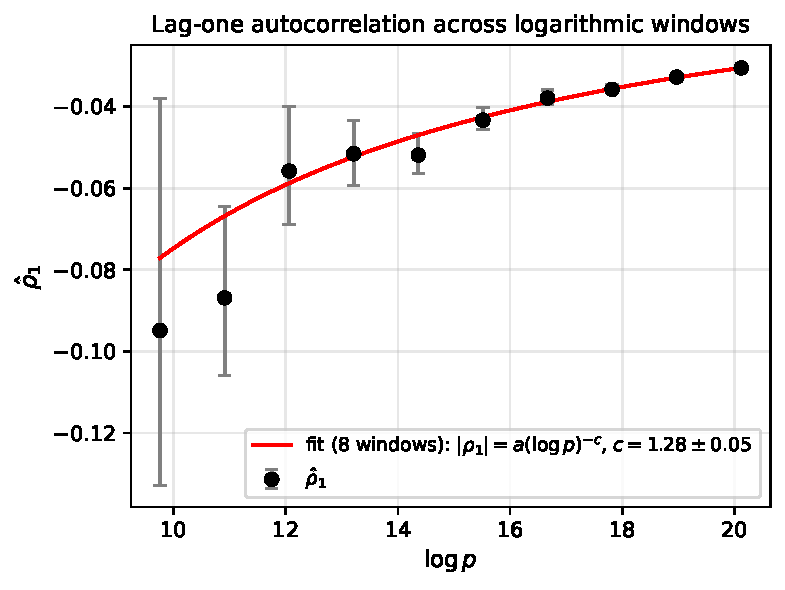
\includegraphics[width=0.65\textwidth]{fig1.pdf}
\caption{Lag-one autocorrelation $\hat\rho_1$ vs.\ $\log p$, with
moving-block bootstrap 95\% CIs and weighted power-law fit
(8 windows, $\log p \ge 12$; $c = 1.28 \pm 0.05$). The two smallest
windows, excluded from the fit, are drawn with open circles.}
\label{fig:rho1}
\end{figure}

\subsection{Ratio structure $\rho_k \approx \rho_1/k$}
\begin{table}[H]\centering
\caption{Ratio $\rho_k / \rho_1$ in $[3\times10^8, 10^9)$.}
\label{tab:ratio}
\begin{tabular}{rrrr}
\toprule
$k$ & $\rho_k / \rho_1$ & $1/k$ & Deviation \\
\midrule
2  & 0.495 & 0.500 & $-1.0\%$ \\
3  & 0.339 & 0.333 & $+1.7\%$ \\
4  & 0.261 & 0.250 & $+4.4\%$ \\
5  & 0.215 & 0.200 & $+7.4\%$ \\
10 & 0.095 & 0.100 & $-4.7\%$ \\
20 & 0.046 & 0.050 & $-7.3\%$ \\
\bottomrule
\end{tabular}
\end{table}

For $k \le 5$ the agreement with $1/k$ is excellent (maximum deviation
$7.4\%$). At larger lags the ratio continues to decay approximately
monotonically but departs from a strict $1/k$ profile; the released
\texttt{correlogram\_v9\_1.csv} contains the full $\rho_k$ vector for
the largest window.

\begin{figure}[H]\centering
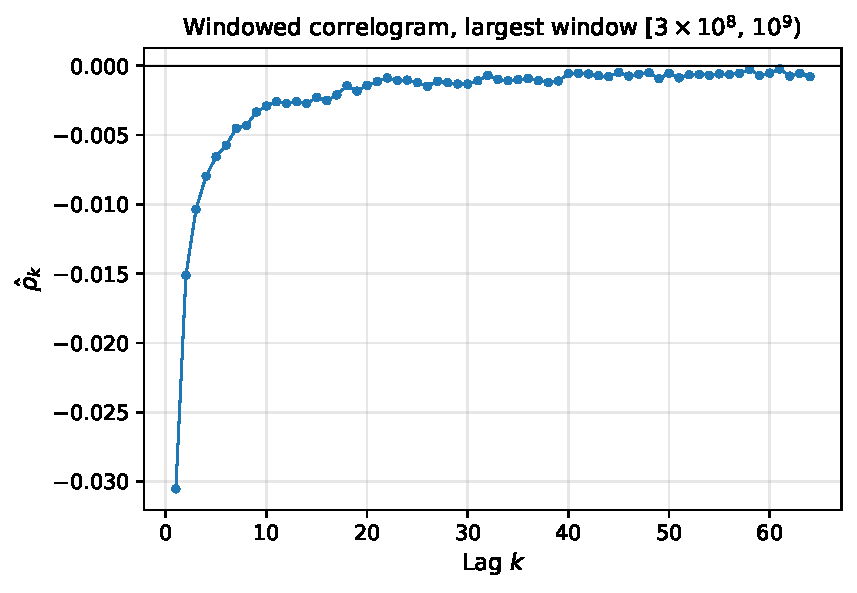
\includegraphics[width=0.75\textwidth]{fig2.pdf}
\caption{Windowed correlogram $\hat\rho_k$ for $k = 1, \ldots, 64$ in
the largest window $[3\times10^8, 10^9)$.}
\label{fig:corr64}
\end{figure}

\subsection{What the result does not claim}
(1)~No universal asymptotic law. (2)~No $\rho_k < 0$ for all $k \le 64$
in every window. (3)~No precise determination of $c$. (4)~No
identification of the mechanism.

% ======================================================================
\section{Modular Conditioning: Approximate Mod-3 Symmetry and Direct
LO-S Test}
\label{sec:mod3}

\subsection{Direct LO-S test}
\begin{table}[H]\centering
\caption{Stay probabilities mod 3 over $[2, 10^9]$.}
\label{tab:los}
\begin{tabular}{lrrrr}
\toprule
Class & $n_{\text{pairs}}$ & $n_{\text{stay}}$ & $P(\text{stay}\mid a)$ & $z$ \\
\midrule
$a = 1$ & 25,422,712 & 11,315,464 & 0.44509 & $-553.7\sigma$ \\
$a = 2$ & 25,424,819 & 11,317,570 & 0.44514 & $-553.3\sigma$ \\
\bottomrule
\end{tabular}
\end{table}

\begin{table}[H]\centering
\caption{Joint $2 \times 2$ table $T[a][b]$.}
\label{tab:joint}
\begin{tabular}{lrr}
\toprule
       & $b = 1$    & $b = 2$    \\
\midrule
$a = 1$ & 11,315,464 & 14,107,248 \\
$a = 2$ & 14,107,249 & 11,317,570 \\
\bottomrule
\end{tabular}
\end{table}

The stay probability is suppressed by $\approx 5.5$ percentage points,
with $z < -553\sigma$. The suppression is the same in the two residue
classes: with the per-class standard errors
$\mathrm{SE} = 9.92 \times 10^{-5}$ tabulated in the released
\texttt{los\_stay\_v10.csv}, the difference
$P(\text{stay}\mid 2) - P(\text{stay}\mid 1) = +4.59 \times 10^{-5}$
corresponds to $z = 0.33$ on a difference standard error of
$\sqrt{\mathrm{SE}_1^2 + \mathrm{SE}_2^2} = 1.40 \times 10^{-4}$ (the two
classes being disjoint, so their estimates are independent), so at the
level of the stay probability the two
classes are statistically indistinguishable. The conditional
autocorrelations of the next subsection do not behave the same way, and
the comparison must be made with care: Table~\ref{tab:los} partitions
by the \emph{opening} prime $p_n$, whereas Table~\ref{tab:cond}
partitions by the \emph{closing} prime $p_{n+1}$
(Section~\ref{sec:data}). These are two different partitions of the gap
sequence, so the two statements are not alternative measurements of one
quantity.

\noindent The $z$-scores above assume independent pairs; since
consecutive pairs share a common prime, the effective sample size is
smaller by a factor of order 2, which would reduce the $z$-scores by
roughly $\sqrt{2}$ while leaving them far above any conventional
significance threshold.

\noindent\textbf{Remark (range-averaged probabilities).} The values
in Table~\ref{tab:los} are aggregated over the full range
$[2, 10^9]$. The LO-S bias is predicted to decay with $p$; a
quantitative test of the conjectured per-class constants $c_1, c_2$
would require adapting the Montgomery--Soundararajan $S_0(H)$
apparatus \cite{MontgomerySoundararajan2004} and is left to future
work.

\noindent\textbf{Remark (relation to $c$).} The predicted mod-3 bias,
a bias in the frequencies of consecutive prime residue classes, scales
like the slowly varying factor
\begin{equation}
f(p) \;=\; \frac{\log\log p}{\log p},
\end{equation}
so that the comparison with a power law in $\log p$ is made by reading
off the local logarithmic slope of $f$:
\begin{equation}
c_{\text{eff}}(p) \;=\; -\frac{\mathrm{d}\log f}
{\mathrm{d}\log(\log p)} \;=\; 1 - \frac{1}{\log\log p},
\label{eq:ceff}
\end{equation}
that is, the exponent for which $f \sim (\log p)^{-c_{\text{eff}}}$ locally.
Over the observed range $[10^4, 10^9]$ this exponent runs from
$c_{\text{eff}} = 0.550$ at $p = 10^4$ to $c_{\text{eff}} = 0.670$ at
$p = 10^9$. Both endpoints lie well below our measured
$c = 1.28$ (bootstrap 95\% CI $[1.14, 1.57]$), so the comparison does
not depend on where in the range one evaluates it. We do not
claim a direct relation between the two exponents: $\rho_1$ measures
correlation of gap \emph{sizes}, whereas the LO-S bias concerns
residue-class mod 3 structure. The fact that both observables follow
power-law decays in $\log p$ is not evidence of a common mechanism,
and we make no such identification.

\subsection{Conditional autocorrelations}
\begin{table}[H]\centering
\caption{Conditional autocorrelations. The lag $k$ is taken
\emph{within} each conditioned subsequence $g^{(1)}$ and $g^{(2)}$ of
Section~\ref{sec:data}, not within the concatenated sequence.}
\label{tab:cond}
\begin{tabular}{rrrr}
\toprule
$k$ & $\rho_{c_1}$ & $\rho_{c_2}$ & Difference \\
\midrule
1  & $-0.016667$ & $-0.015661$ & $-0.001006$ \\
2  & $-0.006707$ & $-0.005442$ & $-0.001265$ \\
3  & $-0.003481$ & $-0.002351$ & $-0.001130$ \\
4  & $-0.000772$ & $-0.001287$ & $+0.000515$ \\
5  & $+0.000318$ & $+0.000192$ & $+0.000127$ \\
\bottomrule
\end{tabular}
\end{table}

\noindent\textbf{The symmetry is approximate, not exact.} Each entry of
Table~\ref{tab:cond} is estimated from $\approx 25.4$ million gaps, so
the white-noise per-class standard error is
$1/\sqrt{n} \approx 1.98 \times 10^{-4}$ and the standard error of a
difference between two independent classes is
$\sqrt{2}/\sqrt{n} \approx 2.80 \times 10^{-4}$. The class differences
at $k = 1, 2, 3$ are therefore $-3.6$, $-4.5$ and $-4.0$ standard
errors. The two residue classes are thus \emph{not} equal in the
literal statistical sense, and ``symmetry'' in the title of this
section is to be read as symmetry up to a statistically significant
but numerically small correction: each difference is at most
$0.0013$ in absolute value. At $k = 4$ and
$k = 5$ the differences shrink to $+1.8$ and $+0.5$ standard errors
and are not significant. We do not model this difference: doing so
would require the two-class constants $c_1, c_2$ of the
Lemke Oliver--Soundararajan conjecture, which we leave open.

\subsection{Numerical coincidence}
$\rho_{c_1, 1} = -0.016667$ coincides with $-1/60$ to four decimals.
Unexplained numerical coincidence; plays no role in any claim.

% ======================================================================
\section{Scaling of $\rho_1$ with $\log p$}\label{sec:scaling}

\begin{table}[H]\centering
\caption{Fitted exponent as a function of window set. The last two
columns are the distances $|c - c_0|/\mathrm{SE}$ to the two hypotheses
of interest, $c_0 = 1$ and $c_0 = 2$, computed from the $c$ and
$\mathrm{SE}$ columns as displayed so that they can be checked by
dividing. Every row excludes both hypotheses. The margin varies by
nearly a factor of four for $c_0 = 2$ ($3.7$ to $14.4$) and by a factor
of two for $c_0 = 1$ ($2.6$ to $5.6$); what varies between rows is by
how much, not whether.}
\label{tab:fitc}
\begin{tabular}{lrrrrrr}
\toprule
Window set & $c$ & SE & $R^2$ & $\sigma_{1}$ & $\sigma_{2}$ \\
\midrule
All 10 windows                     & 1.57 & 0.117 & 0.958 & 4.9 & 3.7 \\
8 windows ($\log p \ge 12$), unweighted & 1.26 & 0.10 & 0.963 & 2.6 & 7.4 \\
\textbf{8 windows, weighted by $m_i$}   & \textbf{1.28} & \textbf{0.05} & \textbf{0.990} & 5.6 & 14.4 \\
6 largest, unweighted              & 1.52 & 0.12 & 0.974 & 4.3 & 4.0 \\
6 windows, weighted by $m_i$       & 1.29 & 0.07 & 0.990 & 4.1 & 10.1 \\
\bottomrule
\end{tabular}
\end{table}

Bootstrap 95\% CI (8 windows, weighted): $[1.14, 1.57]$. Varying the
choice of window set (from 6 to 10 windows, weighted or unweighted)
produces point estimates of $c$ ranging from 1.26 to 1.57; this
systematic sensitivity should be considered alongside the statistical
bootstrap interval when interpreting the value of $c$.

\begin{table}[H]\centering
\caption{Conclusions by hypothesis. The $\sigma$-values quoted in the
middle column use the weighted 8-window fit standard error $\mathrm{SE}
= 0.05$ as the reference. Under other window-set choices the distance
to $c = 1$ ranges from $2.6\sigma$ to $4.3\sigma$; on the bootstrap
scale of the single fitted row that carries a bootstrap interval,
$\mathrm{SE}_{\text{boot}} \approx 0.11$, the distance to $c = 1$ is
only $2.5\sigma$ (see text below). The distance to $c = 2$ is smaller
than $14.4\sigma$ for every other choice of window set: it ranges from
$3.7\sigma$ to $14.4\sigma$ across the five rows of
Table~\ref{tab:fitc}, and is $6.6\sigma$ on the bootstrap scale.}
\label{tab:robust}
\begin{tabular}{lll}
\toprule
Hypothesis & Distance from $c = 1.28$ & Verdict \\
\midrule
$c = 1$ (naive logarithmic) & $5.6\sigma$ (weighted)  & \textbf{Excluded, suggestively} \\
$c = 2$ (quadratic)         & $14.4\sigma$ (weighted) & \textbf{Excluded} \\
\bottomrule
\end{tabular}
\end{table}

We report $c = 1.28 \pm 0.05$ (statistical, weighted) as the primary
estimate. The corresponding distance of $c = 1$ from the point
estimate depends on the choice of window set: $5.6\sigma$ with the
weighted 8-window fit (SE = 0.05), $4.1\sigma$ with the 6 largest
windows weighted by $m_i$ (SE = 0.07), $4.3\sigma$ with the 6 largest
windows unweighted (SE = 0.12), $4.9\sigma$ with all 10 windows
unweighted (SE = 0.117), and $2.6\sigma$ with the unweighted 8-window
fit (SE = 0.10). The last two columns of Table~\ref{tab:fitc} give all
five figures, and the distances to $c = 2$ alongside them. In every case
tested $c = 1$ lies below the fitted value $c = 1.28$, and it lies
below the lower edge of the one bootstrap interval we computed,
$[1.14, 1.57]$.

That interval is available for the weighted 8-window fit only; the
other rows of Table~\ref{tab:fitc} carry no bootstrap interval, so for
them the comparison is against the fitted value alone. Taking its
half-width as a normal interval, the implied bootstrap standard error
is
$\mathrm{SE}_{\text{boot}} = (1.57 - 1.14)/(2 \times 1.96) \approx
0.11$, which is more than twice the weighted-fit standard error of
$0.05$ quoted above. On the bootstrap scale the distance from the point
estimate $c = 1.28$ to $c = 1$ is therefore
$(1.28 - 1.00)/0.11 \approx 2.5\sigma$, not the $5.6\sigma$ obtained
from the weighted-fit standard error. The margin is thus modest, and we
characterize the exclusion of $c = 1$ as suggestive: it holds for every
window set we tested, but not uniformly strongly, and the bootstrap
standard error is the more conservative of the two. The exclusion of
$c = 2$ is by contrast more robust: it ranges from $3.7\sigma$ (all
10 windows, unweighted) to $14.4\sigma$ (the weighted 8-window fit), and
is $6.6\sigma$ on the bootstrap scale. Even the weakest of the five
window sets excludes $c = 2$, but a reader should quote the range rather
than the upper end of it.

% ======================================================================
\section{Pair Ratios and the Hardy--Littlewood Baseline}\label{sec:pair}

The use of pair correlations as a probe of number-theoretic structure
follows the classical analysis of the pair correlation of zeros of
the zeta function \cite{Montgomery1973} and the distribution of
spacings between such zeros \cite{Odlyzko1987}; we apply the same
pairwise viewpoint to the primes themselves.

\begin{table}[H]\centering
\caption{Observed, HL, and IE pair ratios at $N = 10^9$.}
\label{tab:pairs}
\begin{tabular}{lrrrrr}
\toprule
$(a,b)$ & $R_{\mathrm{obs}}$ & $R_{\mathrm{HL}}$ & $R_{\mathrm{model}}$ & rel.\ err.\ HL & rel.\ err.\ IE \\
\midrule
(2, 10) & 1.9586 & 1.8446 & 1.9460 & $-5.82\%$ & $-0.64\%$ \\
(10, 2) & 1.9567 & 1.8446 & 1.9460 & $-5.73\%$ & $-0.55\%$ \\
(2, 28) & 2.7086 & 2.5619 & 2.7035 & $-5.42\%$ & $-0.19\%$ \\
(28, 2) & 2.7184 & 2.5619 & 2.7035 & $-5.76\%$ & $-0.55\%$ \\
(14, 16) & 2.5434 & 2.5619 & 2.5422 & $+0.73\%$ & $-0.05\%$ \\
(16, 14) & 2.5408 & 2.5619 & 2.5422 & $+0.83\%$ & $+0.06\%$ \\
(26, 4) & 2.6254 & 2.4799 & 2.6114 & $-5.54\%$ & $-0.53\%$ \\
(4, 26) & 2.6118 & 2.4799 & 2.6114 & $-5.05\%$ & $-0.01\%$ \\
(6, 6) & 0.8162 & 0.8198 & 0.8157 & $+0.44\%$ & $-0.05\%$ \\
(6, 12) & 0.8750 & 0.8198 & 0.8706 & $-6.31\%$ & $-0.50\%$ \\
(12, 6) & 0.8722 & 0.8198 & 0.8706 & $-6.00\%$ & $-0.18\%$ \\
(6, 4) & 1.2511 & 1.2297 & 1.2448 & $-1.71\%$ & $-0.50\%$ \\
(4, 6) & 1.2509 & 1.2297 & 1.2448 & $-1.69\%$ & $-0.48\%$ \\
(2, 4) & 1.6454 & 1.6396 & 1.6396 & $-0.35\%$ & $-0.35\%$ \\
(4, 2) & 1.6464 & 1.6396 & 1.6396 & $-0.42\%$ & $-0.42\%$ \\
(2, 6) & 0.8564 & 0.8198 & 0.8513 & $-4.28\%$ & $-0.60\%$ \\
(6, 2) & 0.8567 & 0.8198 & 0.8513 & $-4.31\%$ & $-0.63\%$ \\
\bottomrule
\end{tabular}
\end{table}

\noindent\textbf{Note on $(2,4)$ and $(4,2)$.} For these two pairs, the
interior set $E_{a,b}$ contains a single element ($h = 4$), so the
inclusion--exclusion sum truncates naturally at $|J| \le 1$, well
within the truncation order $R = 4$. Hence $R_{\mathrm{model}} =
R_{\mathrm{HL}}$ exactly for these pairs. The residual $\approx
0.35\%$ is therefore \emph{not} attributable to truncation, but
reflects the intrinsic finite-$N$ deviation of the naive HL heuristic:
$\hat R_{\mathrm{obs}}$ weights the range $x \in [2, 10^9]$ with
density $\propto 1/\log x$, giving more weight to small $x$ where HL
corrections are large, whereas $R_{\mathrm{HL}}$ is a local
prediction. This is an inherent scale-mixing bias within the model.

\begin{table}[H]\centering
\caption{Summary statistics.}
\label{tab:pairsummary}
\begin{tabular}{lrr}
\toprule
Metric & Naive HL & IE Model \\
\midrule
Mean abs.\ rel.\ error & 3.55\% & \textbf{0.37\%} \\
Max abs.\ rel.\ error  & 6.31\% & 0.64\% \\
Improvement factor     & ---    & \textbf{9.6$\times$} \\
\bottomrule
\end{tabular}
\end{table}

\begin{figure}[H]\centering
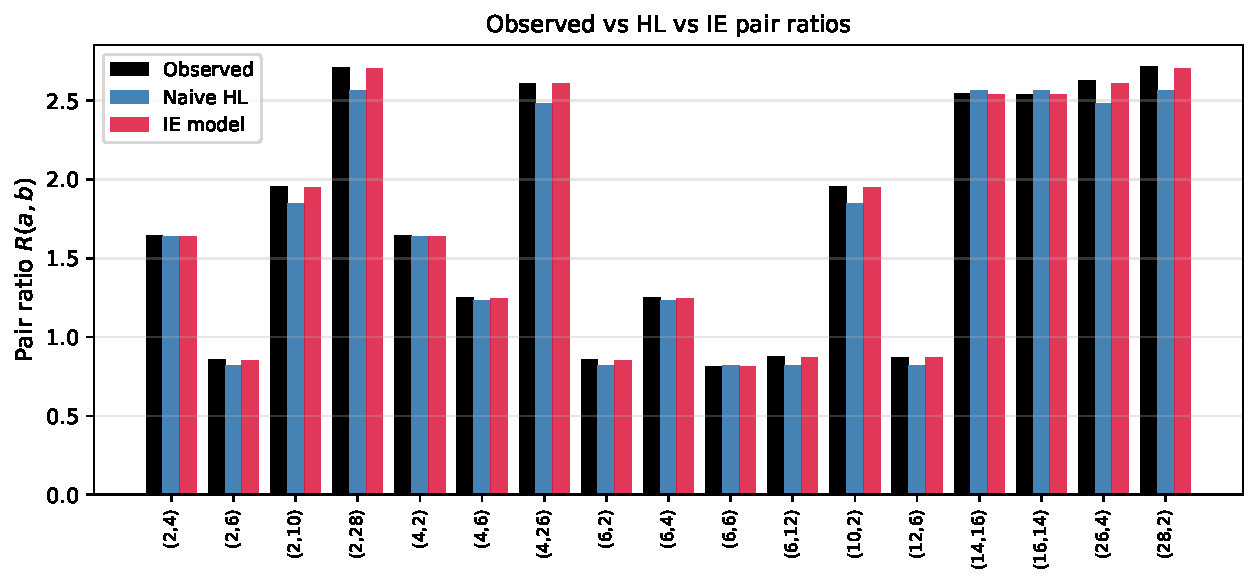
\includegraphics[width=0.9\textwidth]{fig5.pdf}
\caption{Observed vs.\ HL vs.\ IE pair ratios.}
\label{fig:pairs}
\end{figure}

% ======================================================================
\section{Limitations and Reproducibility}\label{sec:limits}

We do not claim: a proof of any asymptotic law; a universal bound
$\rho_k < 0$ for all $k \le 64$; a quantitative test of the LO-S
conjecture at the level of the $c_1, c_2$ coefficients; a
rigorous theorem-level pair-ratio formula.

Methodological caveats: non-stationarity and windowing; choice of
detrending; choice of window boundaries; bootstrap block length;
permutation test scope
($K = 10$ only); the sign statistic in Section~\ref{sec:global} is
indicative but does not constitute an independent significance test;
the mod-3 symmetry of Section~\ref{sec:mod3} is approximate, and the
two residue classes differ significantly in their conditional
autocorrelations at $k \leq 4$, under the closing-prime partition,
which is not the opening-prime partition used for the LO-S
contingency table; the exclusion of $c = 1$ is suggestive rather than
decisive, and rests on a bootstrap interval available for one window
set only; the value $\psi(10^9) - 10^9 = +1{,}595.99$ reported in
Appendix~A is a byproduct of our own pipeline, cross-checked against a
second computation of our own rather than against a tabulated
reference, and quoted to the precision that check supports.

\subsection{Data and code availability}
All code, CSV outputs, and a \texttt{README} are available at
\url{\RepoURL}.

\subsection{Computational cost}
\begin{table}[H]\centering
\caption{Computational cost at $N = 10^9$.}
\label{tab:cost}
\begin{tabular}{lr}
\toprule
Stage & Time (s) \\
\midrule
Sieve & 122 \\
Bootstrap ($B = 5000$, $K = 64$) & 67,310 \\
Permutation ($P = 2000$, $K = 10$) & 9,650 \\
Mod-3 + correlogram ($K = 64$) & 30 \\
\textbf{v9.1 subtotal} & \textbf{77,112} \\
Global correlogram $K = 1024$ on $\delta$ & 539 \\
Global correlogram $K = 1024$ on raw & 541 \\
LO-S stay + $\rho_k/\rho_1$ & 10 \\
\textbf{v10\_supplement subtotal} & \textbf{1,090} \\
\textbf{Total} & \textbf{78,202 s $\approx$ 21.7 h} \\
\bottomrule
\end{tabular}
\end{table}

% ======================================================================
\clearpage
\section*{References}\label{sec:refs}
\addcontentsline{toc}{section}{References}
\bibliographystyle{plain}
\bibliography{refs}

% ======================================================================
\section{Acknowledgments and AI Disclosure}\label{sec:ack}

\subsection{Contributions}
\textbf{Claude (Anthropic).} Identification of the non-stationarity
artifact; review of the bootstrap methodology; methodological review.

{\emergencystretch=2em
\textbf{Kimi (Moonshot AI).} Inclusion--exclusion model
(Section~\ref{sec:pair}); telescoping identity (Appendix~A); prediction
of the $K = 1024$ correlogram statistics; $\rho_k/\rho_1$ ratio
structure. Independent numerical verification of $\pi(10^9)$, $P$,
$\psi(10^9) - 10^9$, and the LO-S stay probabilities is also
acknowledged.\par}

Neither AI system is listed as an author.

\subsection{AI Disclosure Statement}
AI-assisted tools (Claude, Anthropic; Kimi, Moonshot AI) were used for
code verification, methodological review, and drafting assistance.
\textbf{The author retains full responsibility for the content,
analysis, and conclusions of this paper.} All numerical results,
tables, and figures have been independently verified by the author
against the released code and data.

\subsection{Data and computing resources}
Single workstation, 4 threads, 12 GB RAM. Total time $\approx 22$~h.
No GPU acceleration.

\subsection{Funding}
No external funding.

% ======================================================================
\appendix

\section{Telescoping Identity and a Byproduct Estimate of
$\psi(10^9) - 10^9$}

Let $\delta_n = g_n - \log p_n$ and $P = 999{,}999{,}937$. Summing:
\begin{equation}
\sum_{n=1}^{n_{\text{gaps}}} \delta_n
= \sum_n g_n - \sum_n \log p_n
= (P - 2) - (\theta(P) - \log P).
\end{equation}
Rearranging:
\begin{equation}
\bar\delta = \frac{P - \theta(P) + \log P - 2}{n_{\text{gaps}}}.
\label{eq:deltabar}
\end{equation}
No approximation is involved.

We evaluate $\theta(P)$ by two independent routes and they agree.

\noindent\emph{Route 1, through $\bar\delta$.} The pipeline works from
the integer gap sequence and reports $\bar\delta_{\text{obs}} =
6.092163 \times 10^{-4}$, seven significant digits. With $\log P =
20.723266$, Eq.~\eqref{eq:deltabar} inverts to
\begin{equation}
P - \theta(P) = 30{,}958.422043 ,
\end{equation}
and with the $\theta$-powers sum
$\sum_{k \ge 2} \theta(\lfloor N^{1/k}\rfloor) = 32{,}617.412861$
obtained from the same run, extraction gives
\begin{equation}
\psi(10^9) - 10^9 = 32{,}617.41 - 30{,}958.42 - 63 = +1{,}595.99 .
\end{equation}
The term $-63 = P - 10^9$ accounts for the offset between the largest
prime $P$ and the sieve limit $10^9$.

\noindent\emph{Route 2, enumerating the primes.} $\theta(P)$ does not
have to be inferred from a rounded mean. A segmented sieve of
Eratosthenes over $[2, 10^9]$ enumerates all $50{,}847{,}534$ primes
below $10^9$ and returns the same $P$; the count reproduces
$\pi(10^k)$ for $k = 4,\dots,9$, and summing $\log p$ over the
enumeration with correctly rounded summation gives
\begin{equation}
\theta(P) = 999{,}968{,}978.577566, \qquad
P - \theta(P) = 30{,}958.422434 .
\label{eq:thetadirect}
\end{equation}
Recomputing the $\theta$-powers sum from the same enumeration, with
integer roots $\lfloor N^{1/k}\rfloor$, gives $32{,}617.412861$, whose
digits shown agree with the value produced independently by the
$\theta$-powers routine of the C++ pipeline. Two checks come out of the
same code: $\theta(10) = 5.347108 = \log 210$, which has a closed form,
and $\theta(1000) = 956.245265$, which is tabulated. Hence
\begin{equation}
\psi(10^9) - 10^9 = +1{,}595.990428 ,
\label{eq:psidirect}
\end{equation}
which we round to $+1{,}595.9904$. The script is
\texttt{compute\_psi.py}, and it runs in about twenty seconds.

\noindent The two routes differ by $3.9\times10^{-4}$. That is exactly
what seven significant digits of $\bar\delta_{\text{obs}}$ are worth:
half a unit in the last place is $\pm 5\times10^{-11}$, Eq.~\eqref{eq:deltabar}
multiplies it by $n_{\text{gaps}} = 50{,}847{,}532$, and
$5\times10^{-11}\times50{,}847{,}532 = 0.0025$ bounds the discrepancy.
The agreement to $3.9\times10^{-4}$, about one sixth of that bound, is
therefore a genuine cross-check of the telescoping identity against the
gap pipeline rather than a coincidence, and it is why we quote
Route~1 only to $+1{,}595.99$ elsewhere in this paper. Route~2 has no
such amplification: its only error is the sub-ulp error of $\log p$ on
each of the $50.8$ million terms, which cancels to about
$1.6\times10^{-11}$, far below the last digit quoted.

The value $\psi(10^9) - 10^9 = +1{,}595.99$ that this identity yields is
consistent with the published explicit bounds for $|\psi(x) - x|$
tabulated by B\"uthe \cite{Buthe2016}: that method is
stated for $4.92\sqrt{x/\log x} \leq T$, i.e.\ $T \approx 3.4
\times 10^4$ at $x = 10^9$, far below the height to which zeros of
$\zeta$ have been rigorously verified, so $x = 10^9$ is covered. We
cite the arXiv:1410.7015 v4 of that paper, whose abstract records a
corrected version adding a missing summand to Theorem~1 while leaving
the explicit bounds of Tables~1 and~2 valid, and notes that a
corrigendum to the journal version was in preparation. The bounds we
use come from those tables and are therefore unaffected, but a reader
comparing against the journal text should be aware that a later
correction exists. The
same author's sharper uniform bound $|\psi(t) - t| \leq 0.94\sqrt{t}$
for $11 < t \leq 10^{19}$, Math.\ Comp.\ \cite{Buthe2018}, arXiv:1511.02032
v2 marked as the final version to appear in Math.\ Comp., gives
$|\psi(10^9) - 10^9| \leq 29{,}725$ at this argument. The check is
therefore consistent with the external literature but is not sharp: the
published bounds are a factor of about $19$ wider than the
$+1{,}595.99$ we obtain. We note that the value above is produced by
our own two computations, not read off a tabulated reference, so this
comparison confirms that the result is not in conflict with published
work rather than independently reproducing it.

% ======================================================================
\section{Synthetic Demonstration of the Non-Stationarity Artifact}

\noindent To demonstrate that the positive plateau in the raw global
correlogram is a general property of non-stationary sequences, we
generated a synthetic sequence
\[
h_n = \log p_n + \eta_n, \qquad
\eta_n \sim \mathcal N(0, \sigma^2)\ \text{i.i.d.},
\]
with $p_n$ approximated by $n\log n$ for $n = 1, \ldots, 10^6$, and
$\sigma = 6$ chosen so that the plateau in the raw correlogram is
clearly visible above the Bonferroni threshold. We do not attempt to
match the *ratio* of the synthetic maximum to threshold to the ratio
observed in the real data (Table~\ref{tab:k1024raw}); the synthetic
sequence is used only to demonstrate the qualitative mechanism. The
sequence was processed through the identical estimator of
Section~\ref{sec:data}: first on $h_n$ (raw), then on
$h_n - \log p_n$ (exactly detrended). The result
(Table~\ref{tab:B1}) shows that the plateau appears in the raw
sequence and vanishes upon detrending --- confirming that it is a
generic consequence of non-stationarity, not a specific feature of
the prime gaps.

\begin{table}[H]\centering
\begin{tabular}{lcc}\toprule
Quantity & Raw $h_n$ & Detrended $\tilde h_n$ \\ \midrule
Total lags & 1024 & 1024 \\
Positive lags & 1024 & 499 \\
First positive lag & 1 & 1 \\
Maximum positive & 5.415e-01 & 3.732e-03 \\
Bonferroni threshold & 4.061e-03 & 4.061e-03 \\
Max / threshold & 133.339 & 0.919 \\
Tail mean ($k\in[160,1024]$) & 5.316e-01 & -2.040e-05 \\
\bottomrule\end{tabular}
\caption{Synthetic non-stationarity control. The raw sequence $h_n = \log p_n + \eta_n$ exhibits a positive plateau analogous to the raw prime-gap correlogram (Table~\ref{tab:k1024raw}); the detrended sequence does not.}
\label{tab:B1}\end{table}


% ======================================================================
\section{Synthetic-Null Control for Mechanical Detrending Bias}

To rule out the possibility that the negative lag-one autocorrelation
$\rho_1$ reported in Section~\ref{sec:main} is a mechanical artifact
of local detrending, we replicated the full pipeline on synthetic
sequences with no structure.

\noindent\textbf{Method.} For each of the 10 windows used in
Section~\ref{sec:main}, we generated $K$ synthetic i.i.d.\ gap
sequences drawn from an Exponential distribution with no lag
dependence. Each was processed through the identical two-parameter OLS
detrending (intercept and slope in $\log p$), identical window
boundaries, and identical autocorrelation estimator.

\noindent\textbf{Theoretical reference.} For an i.i.d.\ sequence of
length $m$ detrended by OLS with $q = 2$ fitted parameters (intercept
and slope), the expected mechanical lag-one autocorrelation of the
residuals is
\begin{equation}
\rho_1^{\text{mech}} \approx -\frac{q}{m-q} = -\frac{2}{m-2}.
\label{eq:mech}
\end{equation}
To see why, write $e = (I - H)y$ with $H$ the OLS hat matrix and
$y$ the raw sequence. Under the null the errors $\varepsilon_n$ are
independent with mean zero and variance $\sigma^2$, so
$\mathbb{E}[\sum_i e_i e_{i+1}] = \sigma^2\sum_{i<m}(-\,h_{i,i+1})$
while
$\mathbb{E}[\sum_i e_i^2] = \sigma^2(m - \operatorname{tr}H)$, giving
\[
\mathbb{E}[\hat\rho_1] = -\,\frac{\sum_{i<m} h_{i,i+1}}{m - q},
\]
since $\operatorname{tr}H = q$. For regressors that vary slowly across
the window --- here a constant and $\log p$ --- we have
$h_{i,i+1} \approx h_{i,i}$, so $\sum_{i<m} h_{i,i+1}
\approx \operatorname{tr}H = q$, which is Eq.~\eqref{eq:mech}. We
checked this on the actual window design matrices: $\operatorname{tr}H
= 2.00000$ exactly and $\sum_{i<m} h_{i,i+1} = 1.998$, $1.999$,
$2.000$, $2.000$ for $m = 2{,}016$, $6{,}347$, $16{,}405$,
$52{,}501$, so Eq.~\eqref{eq:mech} is accurate to $0.1\%$ in the
smallest window and better than $0.01\%$ thereafter. Eq.~\eqref{eq:mech}
is a controlled approximation for smooth regressors, not a general law
for arbitrary regressors; it is stated here only for the constant and
$\log p$ pair used throughout. The predicted magnitudes were also
verified against direct simulation for the four smallest windows.

\begin{table}[H]\centering
\caption{Synthetic-null control for the ten windows of
Section~\ref{sec:main}. The excess factor is computed against the
closed-form theoretical reference $-2/(m-2)$; the simulated null is
reported separately for the four smallest windows as a check on
higher-order finite-$m$ corrections.}
\label{tab:C1}
\small
\begin{tabular}{lrrrrr}
\toprule
Window & $m$ & Simulated null & Theoretical & Observed & Excess \\
       &     & $\pm$ SEM      & $-2/(m-2)$  & $\rho_1$ & factor \\
\midrule
W1 $[10^4,3\cdot10^4)$       & 2,016      & $-0.001724 \pm 0.000350$ & $-0.000993$ & $-0.09490$ & $95.6\times$ \\
W2 $[3\cdot10^4,10^5)$       & 6,347      & $-0.000047 \pm 0.000228$ & $-0.000315$ & $-0.08688$ & $275.6\times$ \\
W3 $[10^5,3\cdot10^5)$       & 16,405     & $+0.000100 \pm 0.000200$ & $-0.000122$ & $-0.05579$ & $457.6\times$ \\
W4 $[3\cdot10^5,10^6)$       & 52,501     & $+0.000246 \pm 0.000199$ & $-0.000038$ & $-0.05156$ & $1{,}353\times$ \\
W5 $[10^6,3\cdot10^6)$       & 138,318    & --- (analytic)           & $-0.0000145$ & $-0.05188$ & $3{,}588\times$ \\
W6 $[3\cdot10^6,10^7)$       & 447,763    & --- (analytic)           & $-0.0000045$ & $-0.04333$ & $9{,}701\times$ \\
W7 $[10^7,3\cdot10^7)$       & 1,193,280  & --- (analytic)           & $-0.0000017$ & $-0.03793$ & $22{,}631\times$ \\
W8 $[3\cdot10^7,10^8)$       & 3,903,596  & --- (analytic)           & $-0.0000005$ & $-0.03578$ & $69{,}835\times$ \\
W9 $[10^8,3\cdot10^8)$       & 10,490,870 & --- (analytic)           & $-0.0000002$ & $-0.03277$ & $171{,}893\times$ \\
W10 $[3\cdot10^8,10^9)$      & 34,595,208 & --- (analytic)           & $-0.0000001$ & $-0.03054$ & $528{,}269\times$ \\
\bottomrule
\end{tabular}
\end{table}

For the four smallest windows the simulated null and the closed-form
$-2/(m-2)$ agree to within simulation noise; for W1 the simulated
null exceeds the first-order formula by $\approx 2$ SEM, consistent
with higher-order finite-$m$ corrections (the \emph{simulated} null is
therefore used as the reference where available). The excess factors
reported above use the closed-form reference throughout, for internal
consistency; using the simulated null for W1 would reduce its excess
factor to $\approx 55\times$. For the six largest windows, the
closed-form bias is already below $1.5 \times 10^{-5}$, more than four
orders of magnitude below the observed values.

\noindent\textbf{Conclusion.} The observed prime-gap values exceed the
null by factors ranging from $96\times$ to over $500{,}000\times$.
Wherever direct Monte Carlo simulation is feasible (W1--W4), the
excess is $\gtrsim 260\sigma$ against the simulated null.
\textbf{The persistent negative lag-one dependence reported in
Section~\ref{sec:main} cannot be attributed to the detrending
procedure.}

% ======================================================================
\end{document}
